\documentclass{standalone}

\usepackage{tikz}
\usepackage{pgfplots}

\usetikzlibrary{calc}
\pgfplotsset{compat=newest}

\begin{document}
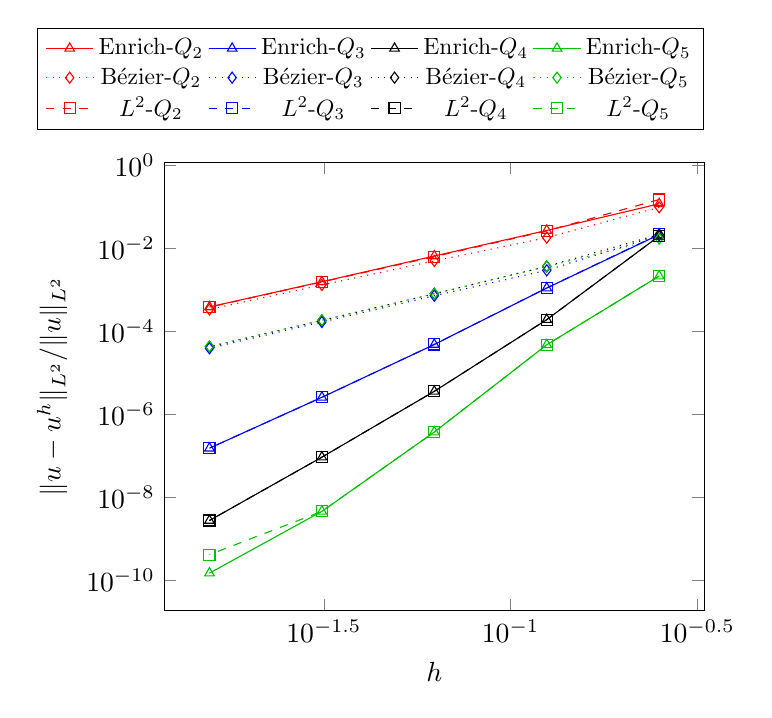
\begin{tikzpicture}
    \begin{loglogaxis}[
        legend columns=4,
    	legend style={at={(1,1.3)}, nodes={scale=.85, transform shape}},
        xlabel=$h$,
        ylabel=${\|u-u^{h}\|_{L^2}}/{\|u\|_{L^2}}$ 
    ]

    \addplot [color=red,mark=triangle] plot coordinates {

        (.25,       0.119565)
        (.125,      0.0273148)
        (.0625,     0.00661773)
        (0.03125,   0.00158961)
        (0.015625,  0.000392298)
    };

    
    \addplot [color=blue,mark=triangle] plot coordinates {

        (.25,       0.021653)
        (.125,      0.00111936)
        (.0625,     4.88932e-05)
        (0.03125,   2.61198e-06)
        (0.015625,  1.55474e-07)
    };

    \addplot [color=black,mark=triangle] plot coordinates {

        (.25,       0.0200108)
        (.125,      0.000193957)
        (.0625,     3.64043e-06)
        (0.03125,   9.44569e-08)
        (0.015625,  2.81632e-09)
    };

    \addplot [color=green!75!black,mark=triangle] plot coordinates {

        (.25,       0.0021764)
        (.125,      4.8063e-05)
        (.0625,     3.80664e-07)
        (0.03125,   4.67219e-09)
        (0.015625,  1.52006e-10)
    };

    
    \addplot [color=red,mark=diamond, every mark/.append style={solid}, dotted] plot coordinates {

        (.25,       0.0983431)
        (.125,      0.0183333)
        (.0625,     0.00503363)
        (0.03125,   0.00133167)
        (0.015625,  0.000341421)
    };

    
    \addplot [color=blue,mark=diamond, every mark/.append style={solid}, dotted] plot coordinates {

        (.25,       0.0209316)
        (.125,      0.00299256)
        (.0625,     0.000729679)
        (0.03125,   0.000169969)
        (0.015625,  0.000039647)
    };

    \addplot [color=black,mark=diamond, every mark/.append style={solid}, dotted] plot coordinates {

        (.25,       0.0218843)
        (.125,      0.00372122)
        (.0625,     0.000814624)
        (0.03125,   0.000185056)
        (0.015625,  0.000043166)
    };

    \addplot [color=green!75!black,mark=diamond, every mark/.append style={solid}, dotted] plot coordinates {

        (.25,       0.0173795)
        (.125,      0.00369684)
        (.0625,     0.000814441)
        (0.03125,   0.000187864)
        (0.015625,  0.000043821)
    };

    
    \addplot [color=red,mark=square, every mark/.append style={solid}, dashed] plot coordinates {

        (.25,       0.151629)
        (.125,      0.0266309)
        (.0625,     0.00638536)
        (0.03125,   0.00156659)
        (0.015625,  0.000388151)
    };

    
    \addplot [color=blue,mark=square, every mark/.append style={solid}, dashed] plot coordinates {

        (.25,       0.0219934)
        (.125,      0.00112746)
        (.0625,     4.90144e-05)
        (0.03125,   2.61451e-06)
        (0.015625,  1.55489e-07)
    };

    \addplot [color=black,mark=square, every mark/.append style={solid}, dashed] plot coordinates {

        (.25,       0.0200278)
        (.125,      0.000194223)
        (.0625,     3.64379e-06)
        (0.03125,   9.44965e-08)
        (0.015625,  2.81381e-09)
    };

    \addplot [color=green!75!black,mark=square, every mark/.append style={solid}, dashed] plot coordinates {

        (.25,       0.0021798)
        (.125,      4.79902e-05)
        (.0625,     3.80295e-07)
        (0.03125,   4.67171e-09)
        (0.015625,  4.24105e-10)
    };

    \logLogSlopeTriangle{0.37}{0.075}{0.2}{6}{green!75!black};
    \logLogSlopeTriangle{0.16}{0.075}{0.18}{5}{black};
    \logLogSlopeTriangle{0.16}{0.075}{0.34}{4}{blue};
    \logLogSlopeTriangle{0.16}{0.075}{0.655}{2}{red};

    \legend{Enrich-$Q_2$\\Enrich-$Q_3$\\Enrich-$Q_4$\\Enrich-$Q_5$\\B\'ezier-$Q_2$\\B\'ezier-$Q_3$\\B\'ezier-$Q_4$\\B\'ezier-$Q_5$\\$L^2$-$Q_2$\\$L^2$-$Q_3$\\$L^2$-$Q_4$\\$L^2$-$Q_5$\\}
    \end{loglogaxis}
\end{tikzpicture}

\end{document}
